\documentclass[../Report.tex]{subfiles}

\begin{document}

\chapter{Implementation and Testing} \label{chap:imp_test}

% \section{Implementation of AI model}

% \section{Implementation of Inference Server}

% \section{Connection between Mobile App and Inference Server}

% \section{Implementation of Mobile App}

% \subsection{User Login}

% \subsection{Database Models}

\section{Testing}

Testing is done both manually and automatically. Manual testing involves running the app and checking if all the features are working as 
intended.\par
Automated testing involves writing test cases that evaluate the functionality of app as small individual parts and later after integration 
as a whole.

% \subsection{AI model accuracy validation}

% \subsection{Testing Inference Server}

% \subsection{Testing UI}

\section{Mobile App Screenshots}
\begin{figure}[H]
    \centering
    \begin{minipage}{.5\textwidth}
      \centering
      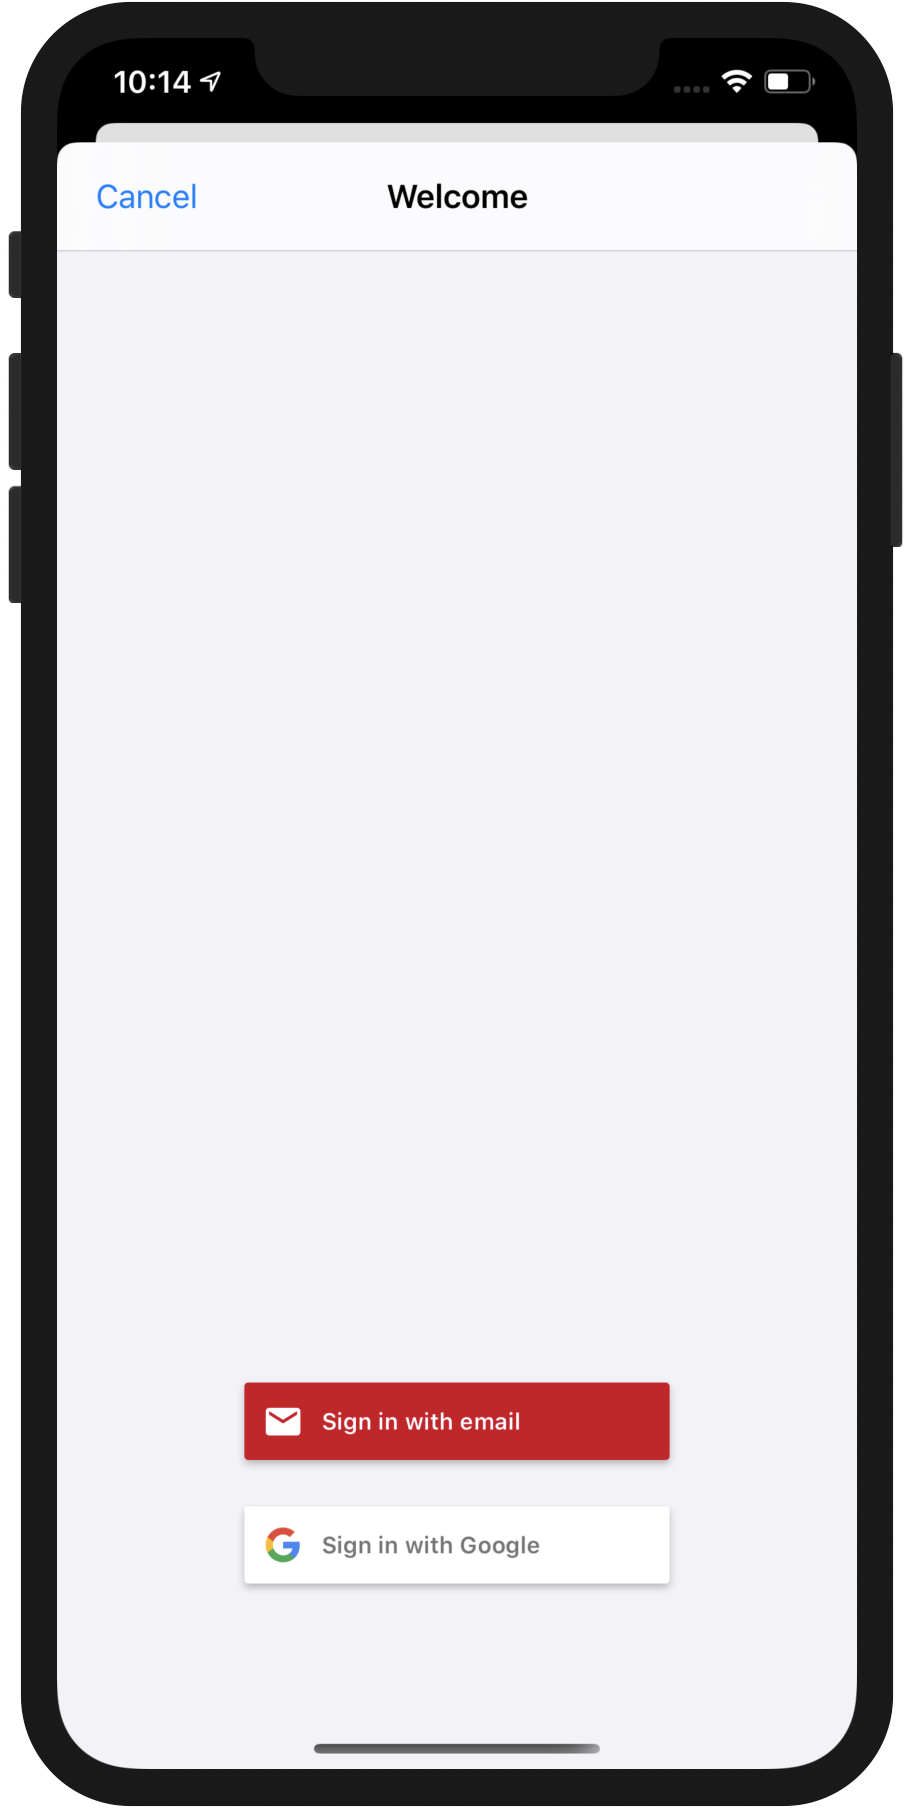
\includegraphics[width=5cm]{images/user_login.png}
      \captionof{figure}{User Login}
      \label{fig:ss_user_login}
    \end{minipage}%
    \begin{minipage}{.5\textwidth}
      \centering
      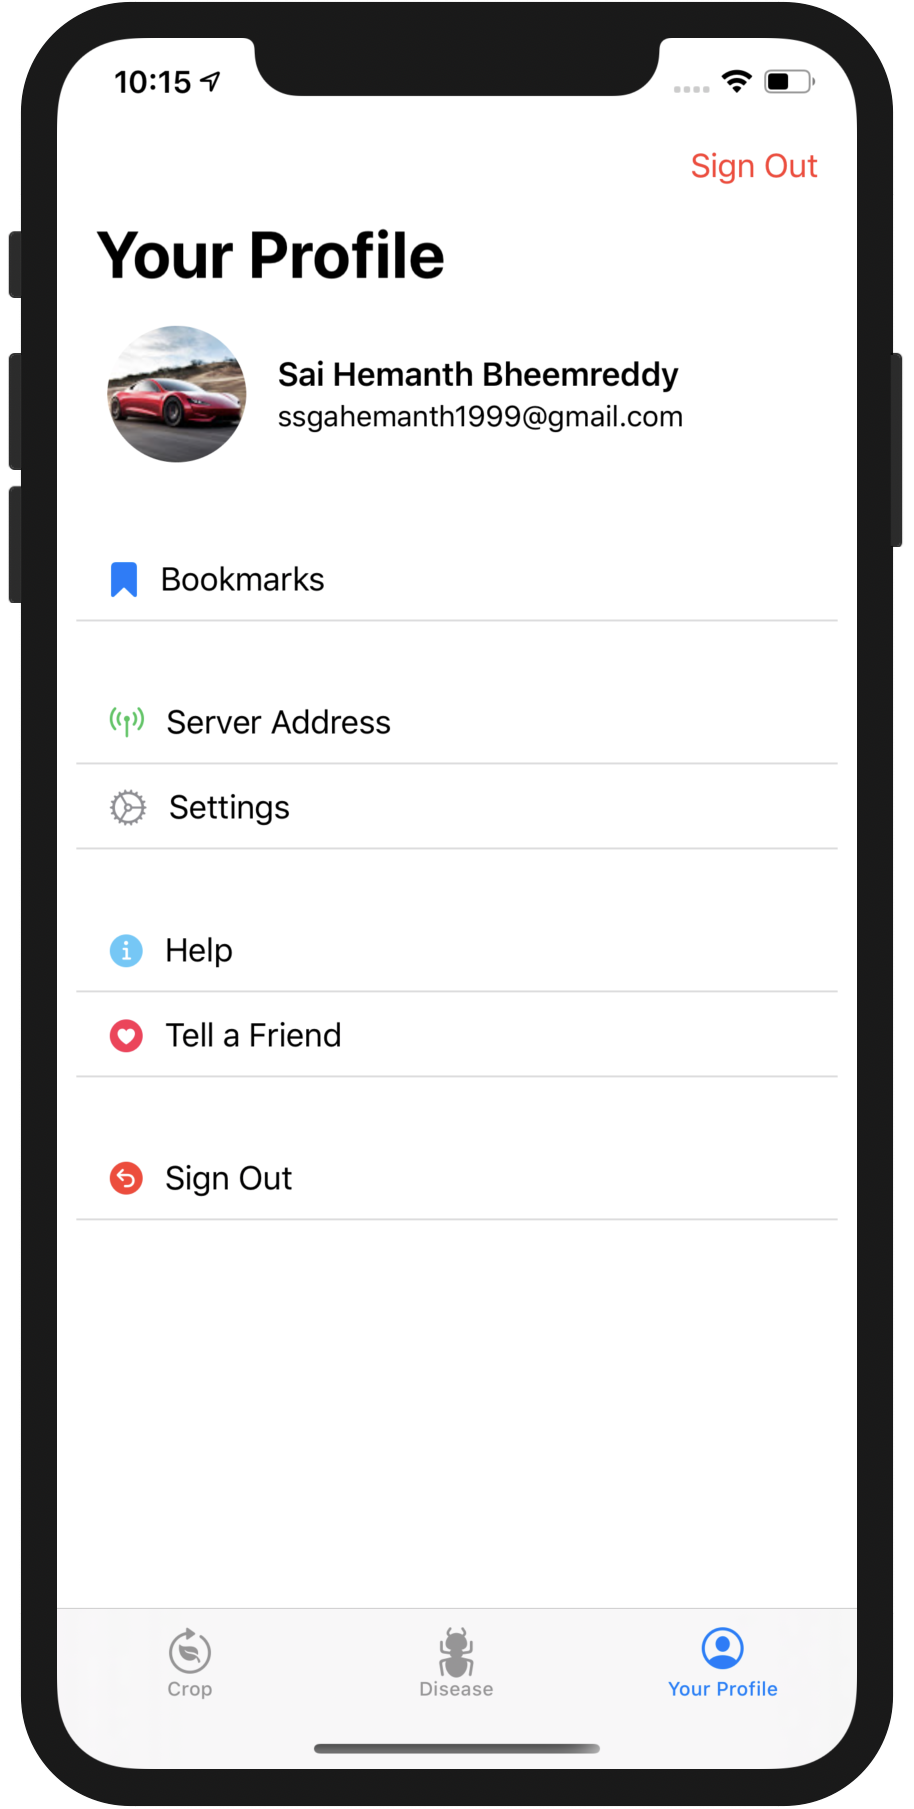
\includegraphics[width=5cm]{images/profile.png}
      \captionof{figure}{User Profile Tab}
      \label{fig:ss_user_profile}
    \end{minipage}
\end{figure}

\noindent When the user first launches the app, the user is asked to login.

\begin{figure}[H]
    \centering
    \begin{minipage}{.5\textwidth}
      \centering
      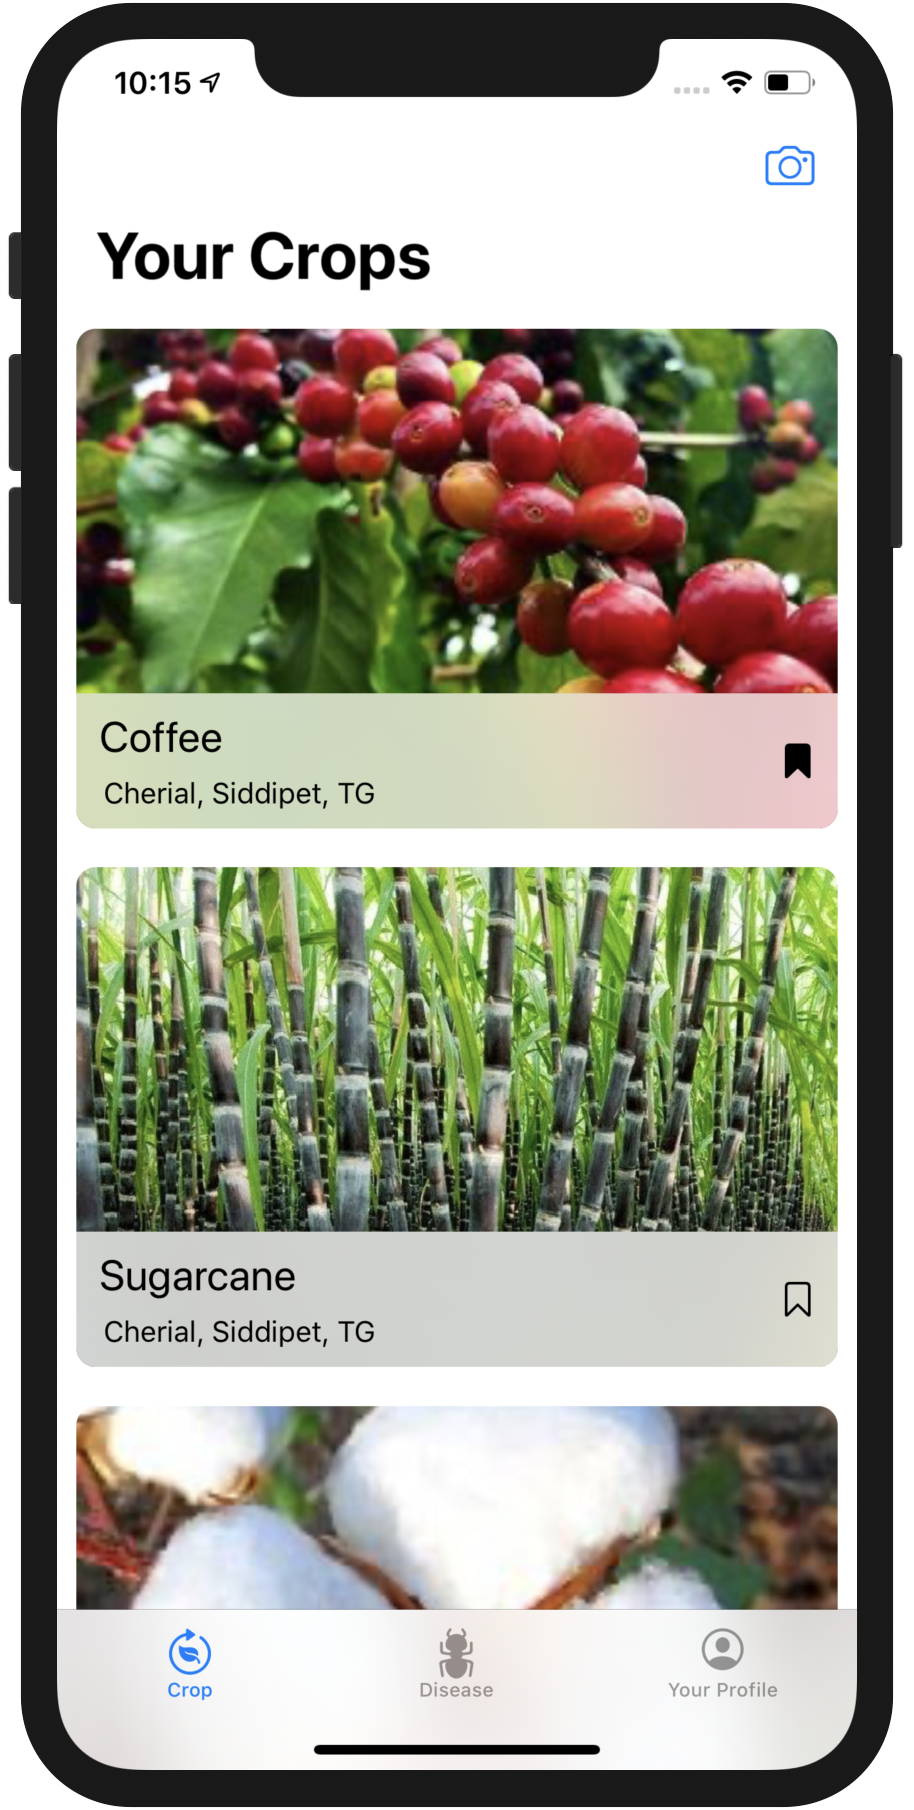
\includegraphics[width=5cm]{images/crop.png}
      \captionof{figure}{Crops Tab}
      \label{fig:ss_crop}
    \end{minipage}%
    \begin{minipage}{.5\textwidth}
      \centering
      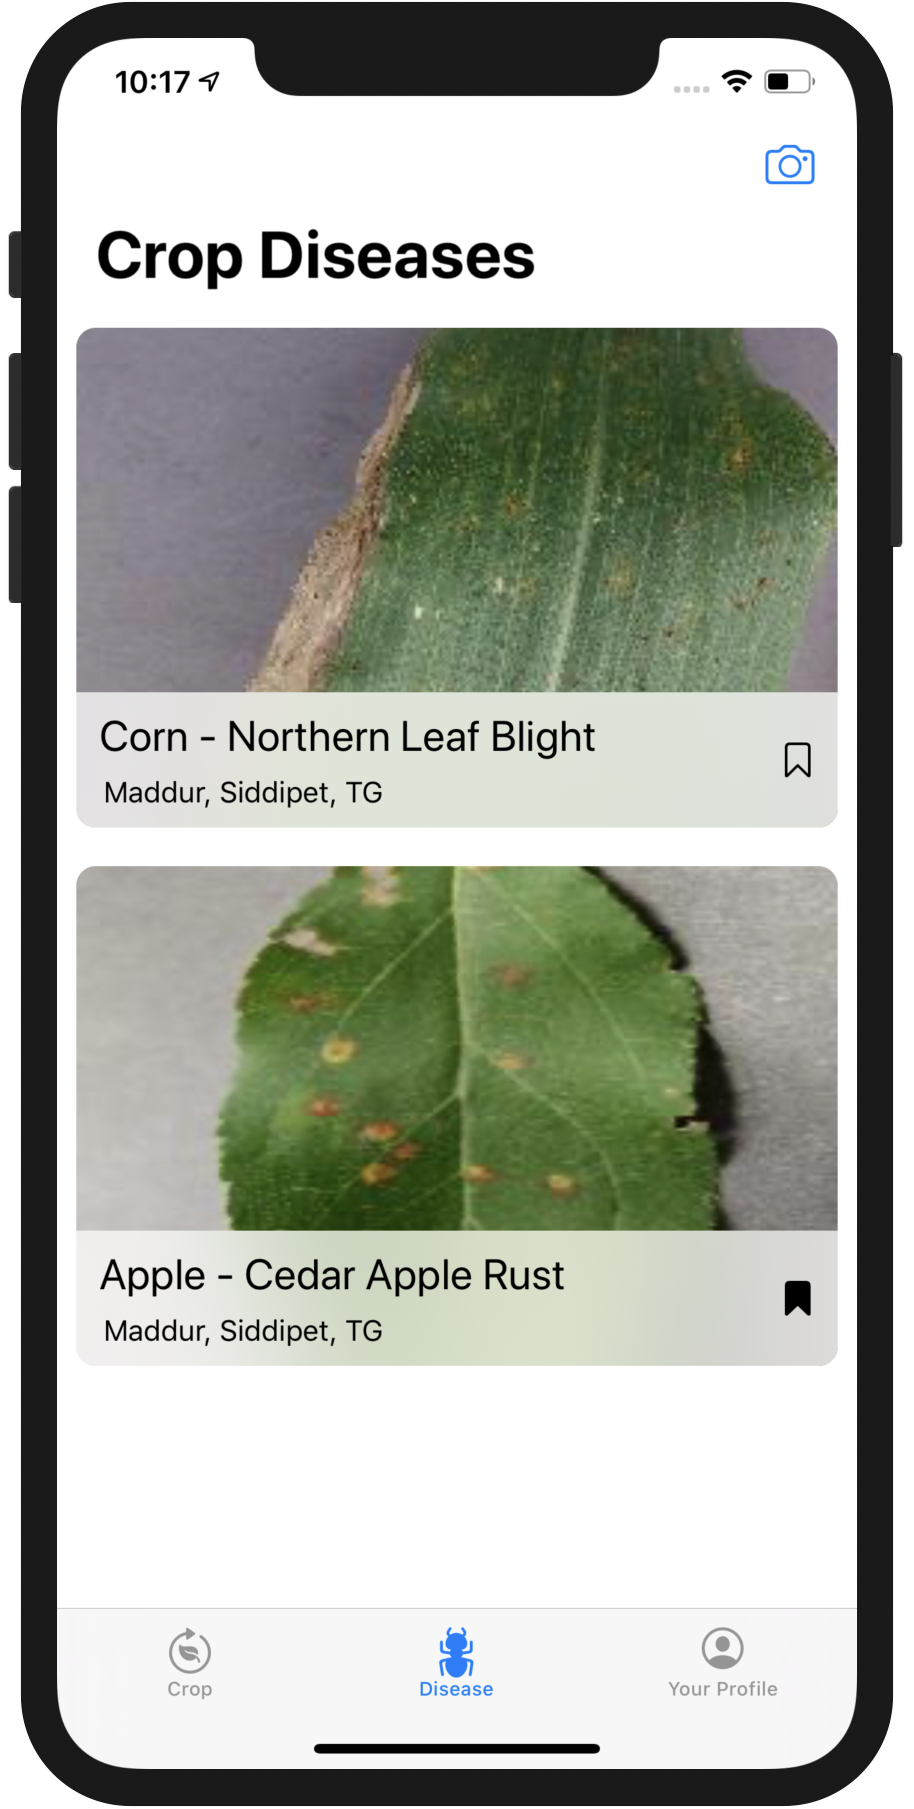
\includegraphics[width=5cm]{images/disease.png}
      \captionof{figure}{Crop Disease Tab}
      \label{fig:ss_disease}
    \end{minipage}
\end{figure}

\noindent These tabs show user's crops and all the information is available within single tap.

\begin{figure}[H]%
    \centering
    \subfloat[label 1]{{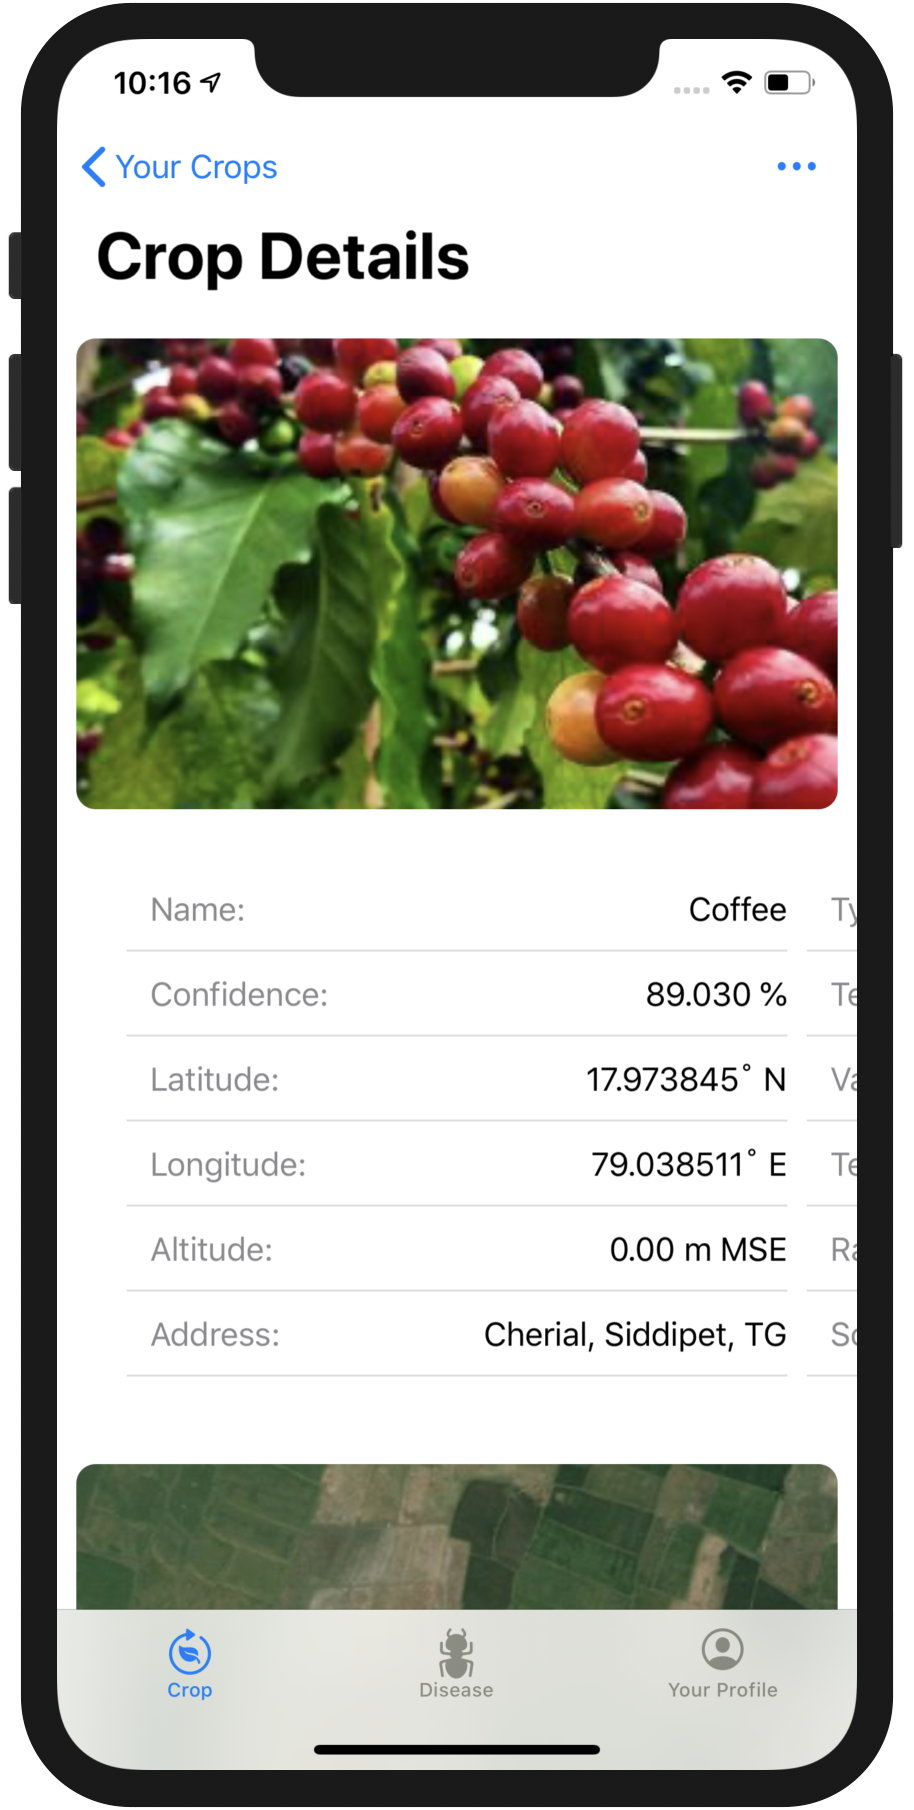
\includegraphics[width=5cm]{images/crop_details_1.png}}}%
    \qquad
    \subfloat[label 2]{{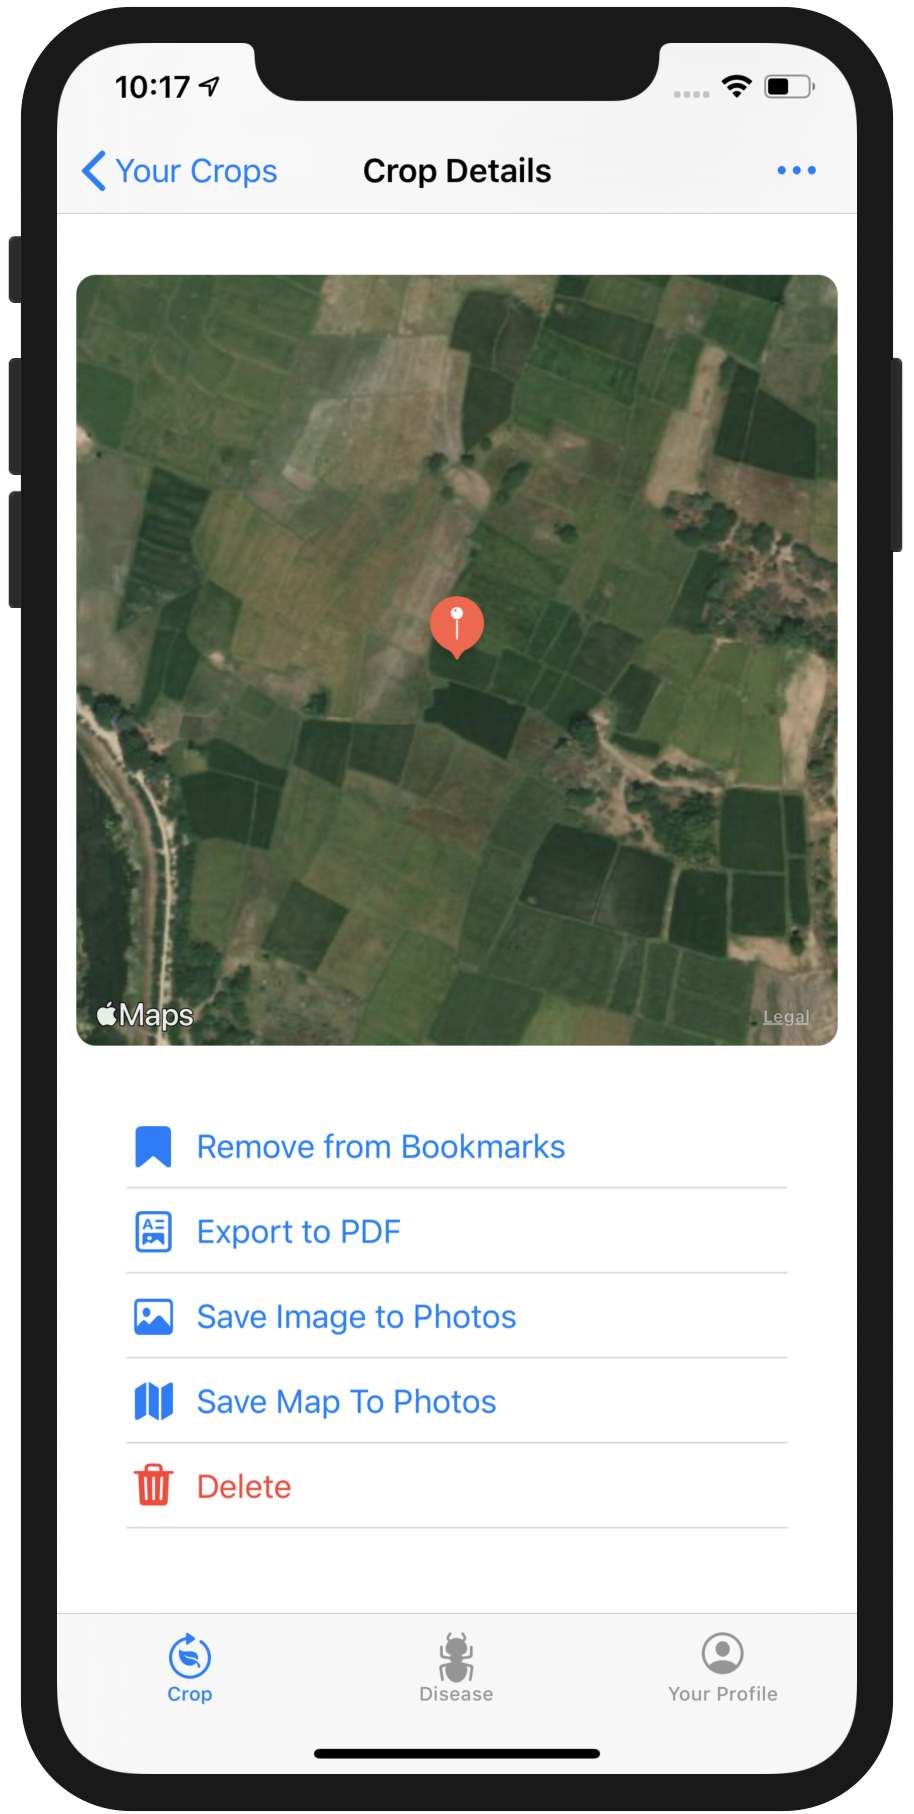
\includegraphics[width=5cm]{images/crop_details_2.png}}}%
    \caption{Crop Details Screen}
    \label{fig:ss_crop_details}%
\end{figure}

\noindent User can tap on any of the card in crop tab to get more details about his crops.

\begin{figure}[H]
    \centering
    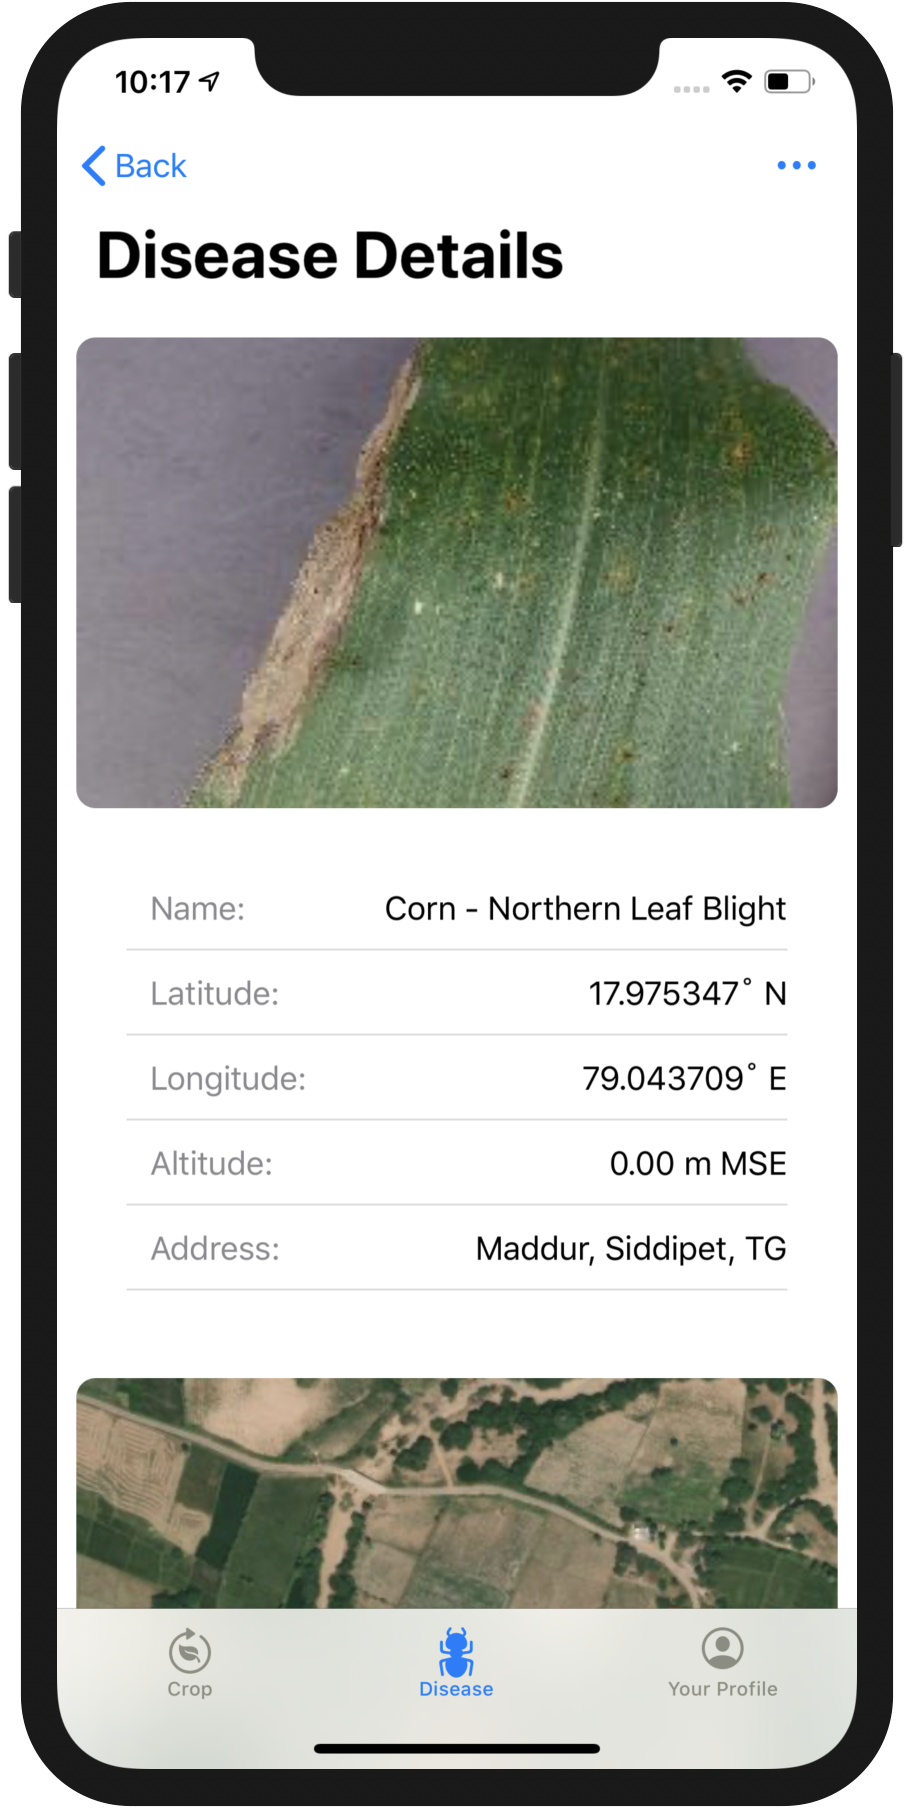
\includegraphics[width=5cm]{images/disease_details.png}
    \caption{Crop Disease Screen}
    \label{fig:ss_disease_details}
\end{figure}

\noindent User can tap on any of the card in disease tab to get more details about his crop disease.

\begin{figure}[H]
    \centering
    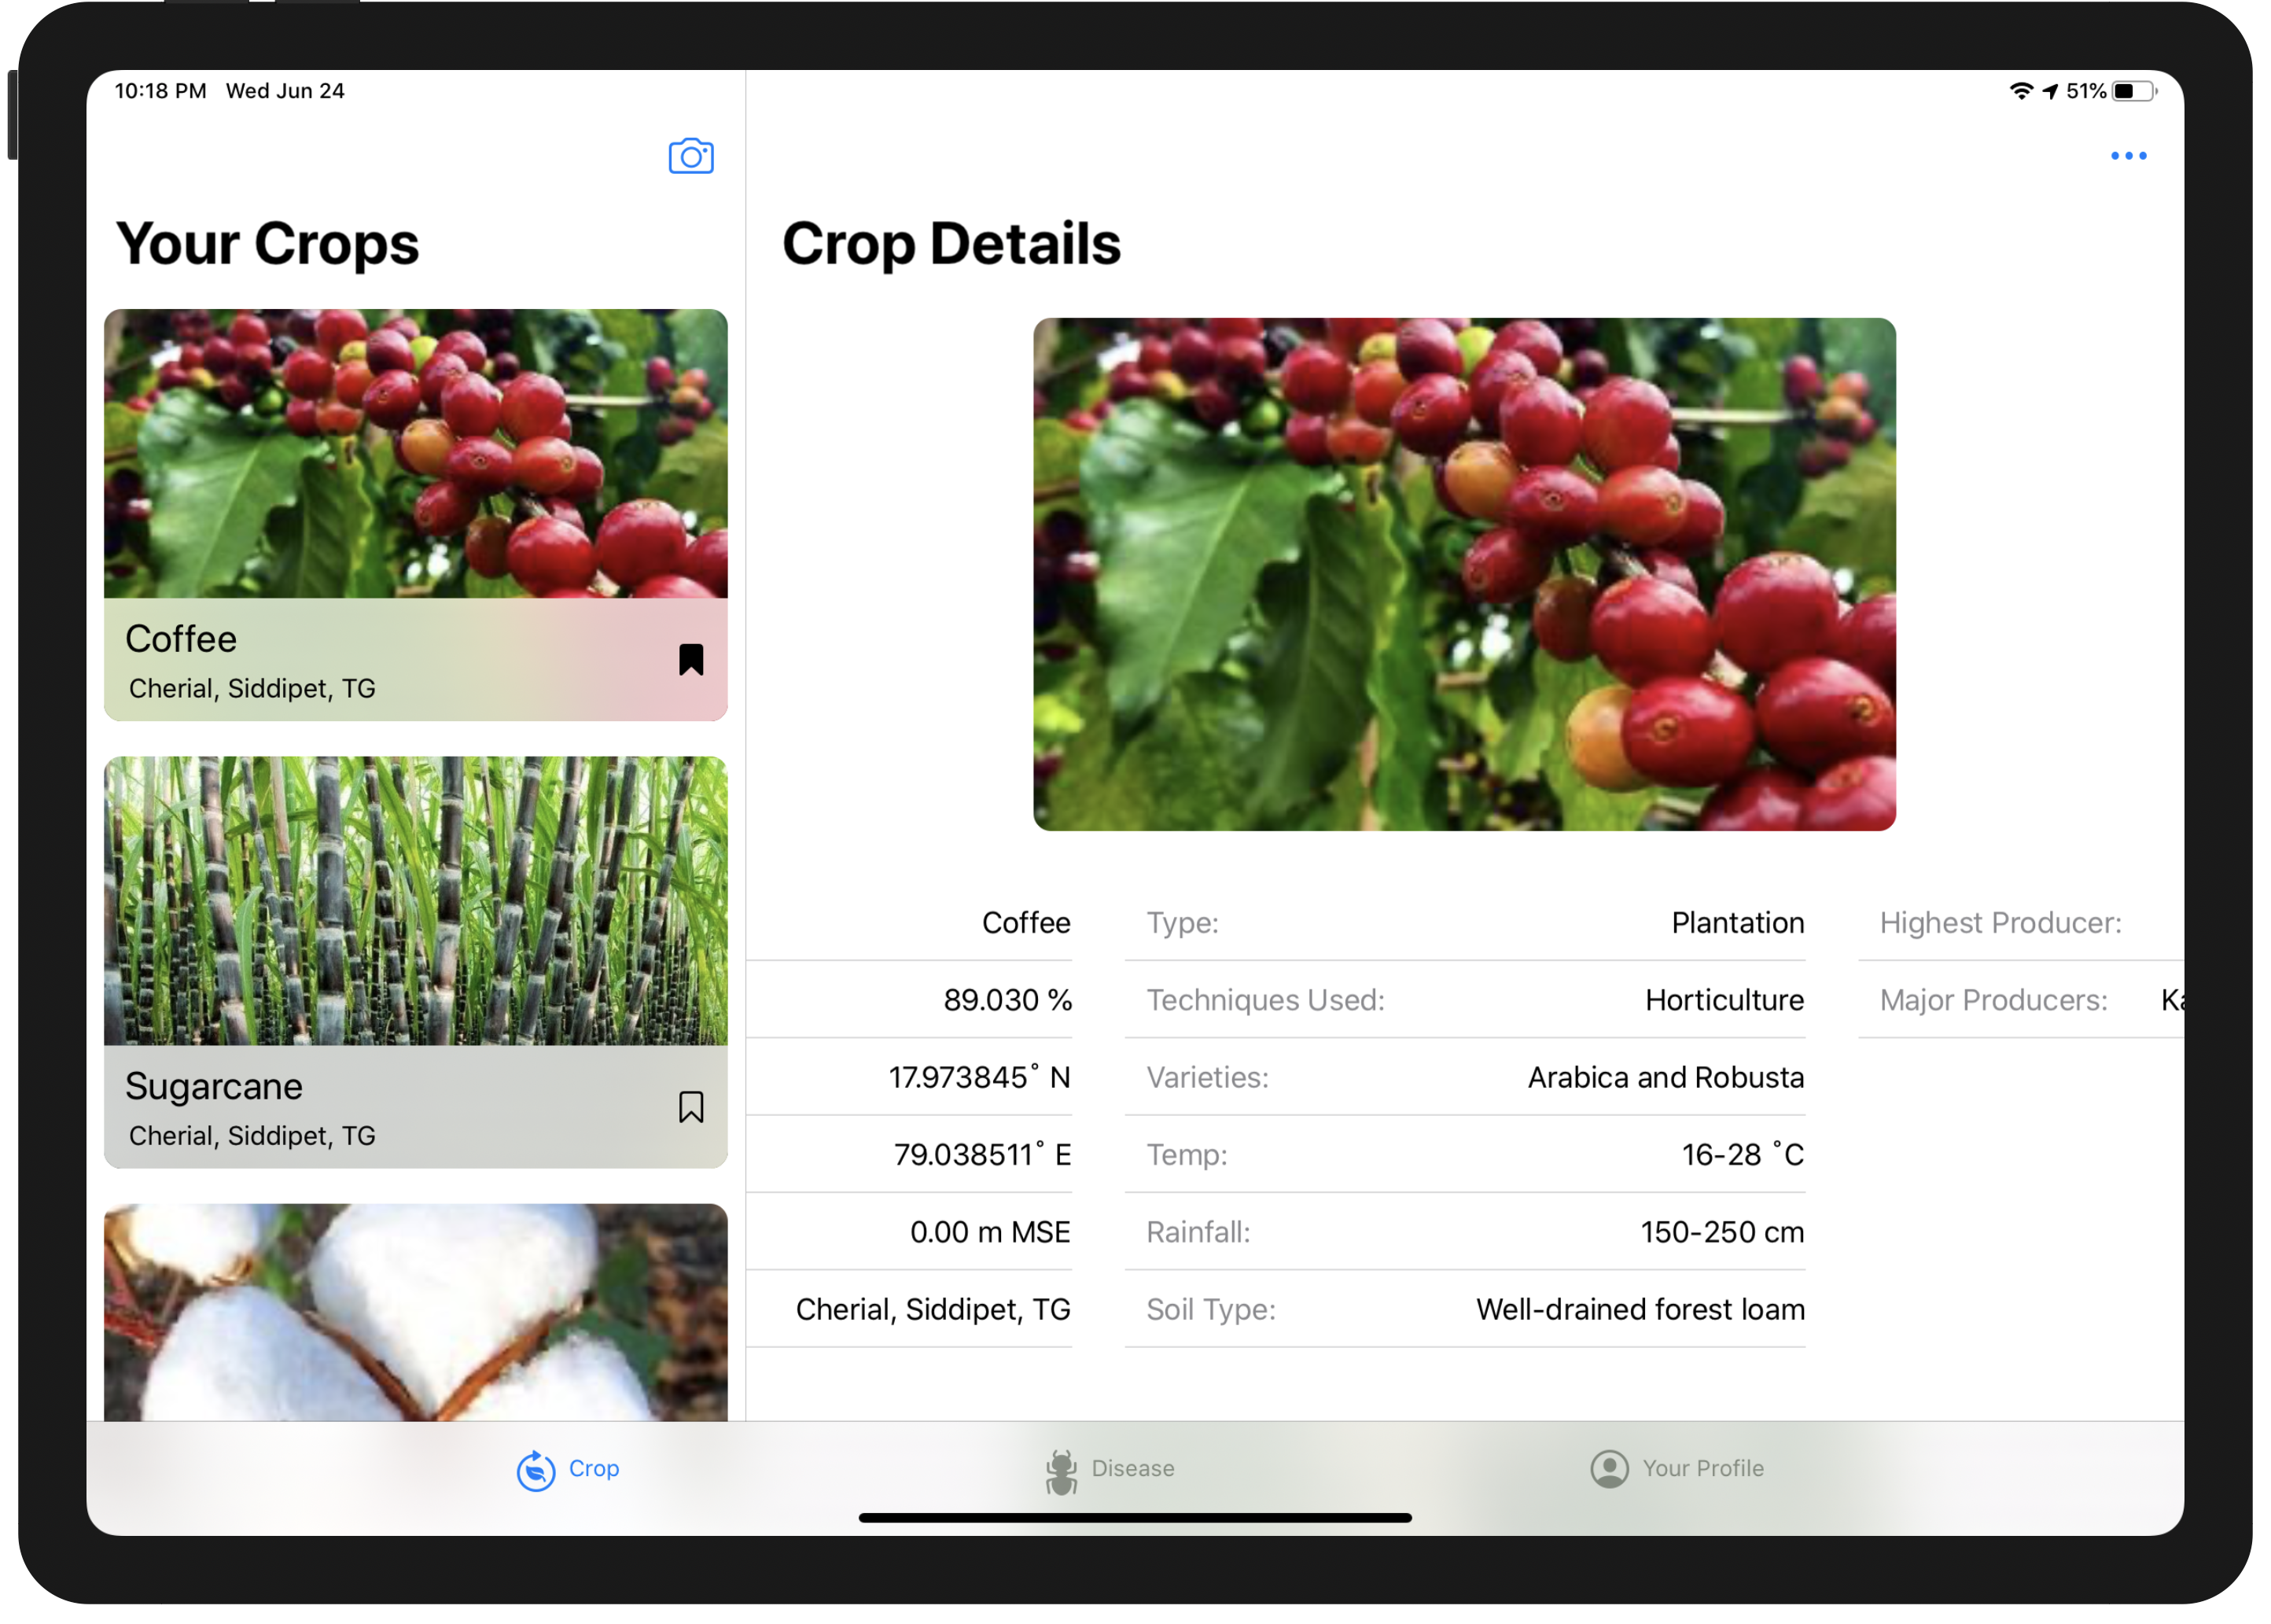
\includegraphics[width=0.75\linewidth]{images/ipad.png}
    \caption{Dynamic UI}
    \label{fig:ss_ipad}
\end{figure}

\noindent The app is made to run on any device and automatically adapts the UI to optimize the screen real estate.

\end{document}